%!TEX root = ../Single-Song.tex
\beginsong{Piratenlied}[wuw={Die Opis}, index={Klingt ein Lied durch die Nacht}]

\markboth{\songtitle}{\songtitle}


\beginverse
\endverse

\centering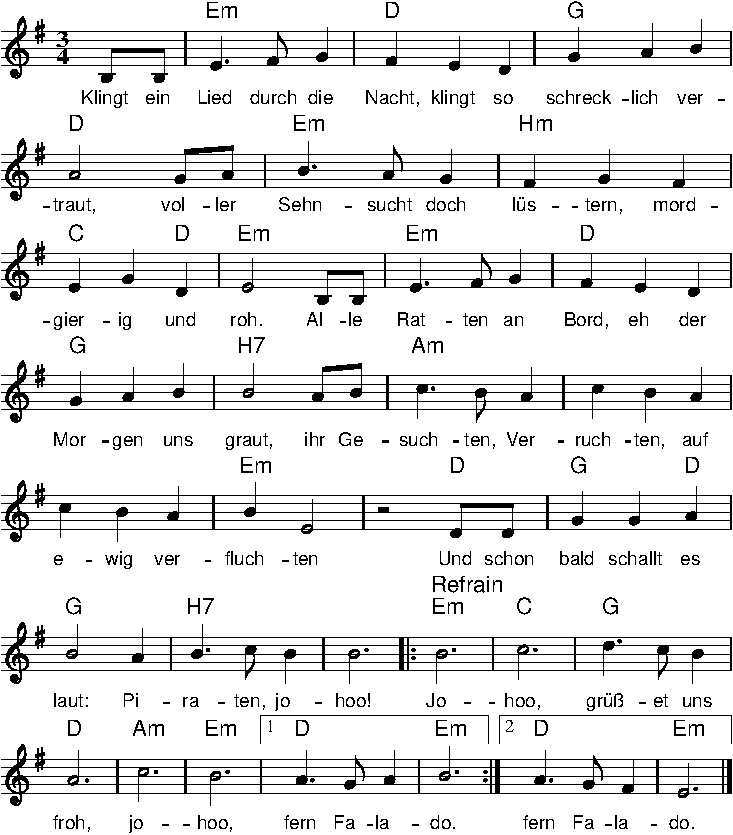
\includegraphics[width=1\textwidth]{Noten/Piratenlied.pdf}	

\beginverse\memorize
Manches \[Em]Heck hat der \[D]Sturm in den \[G]Kurs uns ge\[D]lenkt, 
Und Queen \[Em]Mary die \[D]machten gleich \[C]dreimal \[D]wir \[Em]froh. 
Selbst der \[Em]stolzen Fre\[D]gatte, die mit \[G]Blei uns bes\[H7]chenkt. 
Winkt der \[Am]Stückpforten Flug, unser Stolz vorn am \[Em]Bug. 
\[D]Hat noch \[G]jede versenkt -- Pi\[H7]raten Johoo. 
\endverse

\beginchorus
\lrep \[Em]Jo\[C]hoo, \[G]grüßet uns \[D]froh, \[Am]jo\[Em]hoo, \[D]fern Fala\[Em]do! \rrep
% \newline
\endchorus
%
% \centering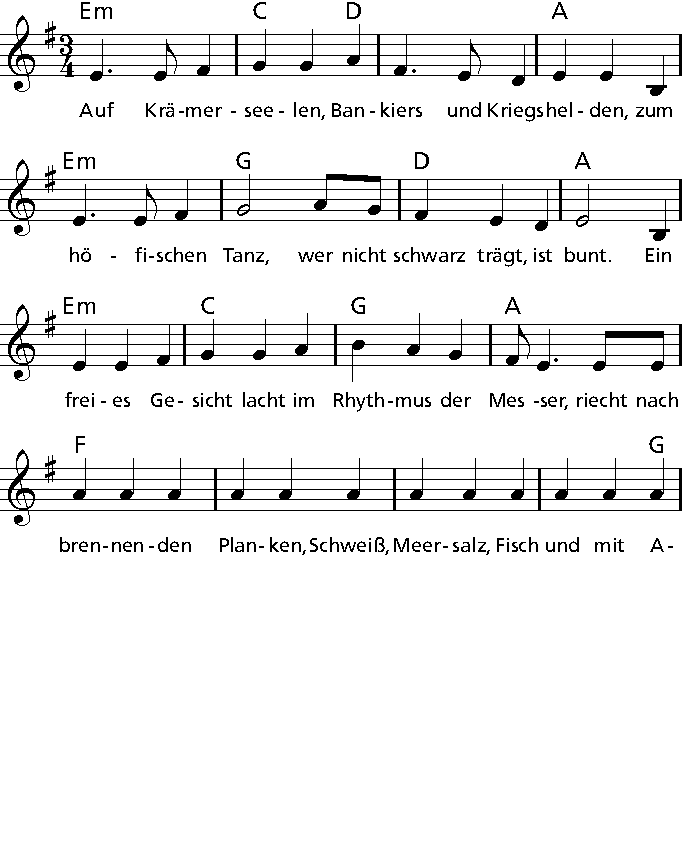
\includegraphics[width=1\textwidth]{Noten/Piratenlied_1a2.pdf}
% \newpage
%
% \centering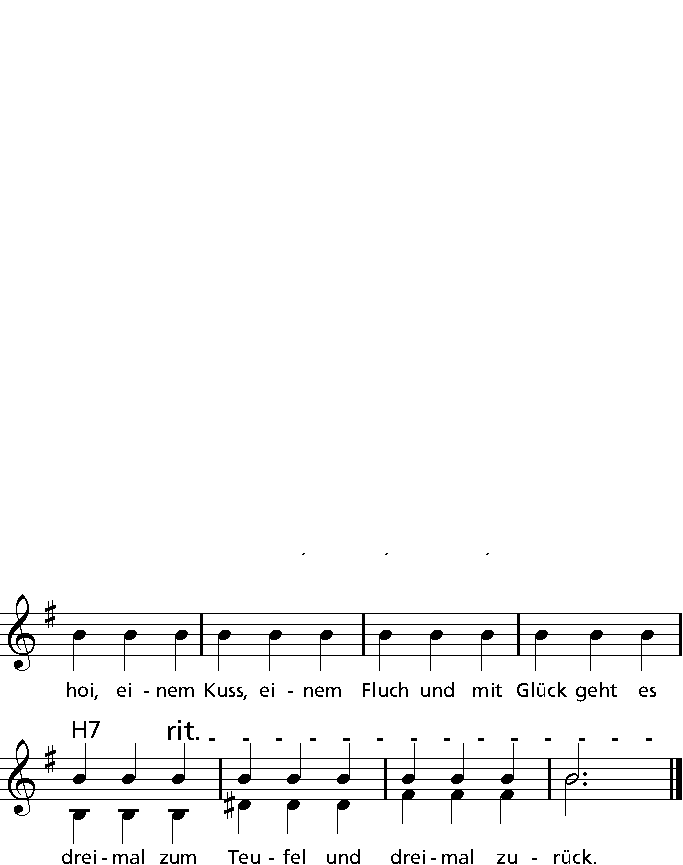
\includegraphics[width=1\textwidth]{Noten/Piratenlied_1b2.pdf}

\beginverse
\[Em]Auf Krämer\[C]seelen, Ban\[D]kiers und Kriegs\[A]helden.
Zum \[Em]höfischen \[C]Tanz -- wer nicht \[D]schwarz trägt ist \[A]bunt.
Ein \[Em]freies Ge\[C]sicht lacht im \[G]Rhythmus der \[D]Messer.
Riecht nach \[F]brennenden Planken, Schweiß, Meersalz, Fisch und mit \[G]Ahoi, einem Kuss, einem Fluch und mit Glück geht es \[H7]dreimal zum Teufel und dreimal zurück.
\endverse

\beginchorus
\lrep \[Em]Jo\[C]hoo, \[G]grüßet uns \[D]froh, \[Am]jo\[Em]hoo, \[D]fern Fala\[Em]do! \rrep
\endchorus

\beginverse
Brüder ^trinkt auf die ^See, die uns ^ruft weit hi^naus, 
Aller ^Sünder Weg ^treiben wir ^ins nir^gend^wo, 
Kehrt doch ^keiner von ^unseren ^Fahrten nach ^Haus. 
Und so ^trinkt auf dies Leben, das bleibt un^vergeben! 
^Und zum ^Ende trinkt aus -- Pi^raten Johoo!
\endverse

% \beginchorus
% \lrep \[Em]Jo\[C]hoo, \[G]grüßet uns \[D]froh, \[Am]jo\[Em]hoo, \[D]fern Fala\[Em]do! \rrep
% \endchorus
%

\endsong

\beginscripture{}

\endscripture

\begin{intersong}

\end{intersong}